We instantiated the above described algorithm in the context of logic grid puzzles. 
In that setting, for $T$, we take $\allconstraints$ for some puzzle $P$, as described in Section \ref{sec:prelims}. There are three types of constraints in $\allconstraints$: transitivity constraints, bijectivity constraints and clues, where the first two follow the same structure in every puzzle and the clues are obtained in a mostly automatic way (see Section \ref{sec:holistic}). 
Before defining a cost-function, and the estimation for $g$ used in our implementation, we provide some observations that drove our design decision. 

\paragraph{Observation 1: Propagations from a single implicit constraint are very easy to understand} Contrary to the clues, the implicit constraints (transitivity/bijectivity) are very limited in form and propagations over them follow well-specified patterns. 
For instance in the case of bijectivity, a typical pattern that occurs is that when $X-1$ out of $X$ possible values for a given function have been derived not to be possible, it is propagated that the last value should be true; this is visualized for instance in Figure \ref{fig:zebrascreen}. 
Hence, in our implementation, we ensure that they are always performed first. Stated differently, $g$ and $f$ are designed in such a way that $g(S_1)\geq f(I,S_2)$ whenever $S_2$ consists of only one implicit constraint and $S_1$ does not. 

\paragraph{Observation 2: Clues propagate rarely by themselves}
We observed that the automatically obtained logic representation of clues usually has quite weak (unit) propagation strength in isolation. 
This is not a property of the clues, but rather of the final obtained translation. As an example, consider the following sentence: 
``The person who ordered capellini is either Damon or Claudia''. From this, a human reasoner might conclude that Angie did not order capellini. 
% The use of the article ``the'' in the above sentence gives away that there is actually a unique person who ordered capellini. 
However, the (automatically) obtained logical representation is 
\[\exists p\in \mathit{person}: \mathit{ordered}(p, \mathit{capellini})\land (p =  \mathit{Damon}\lor p =  \mathit{Claudia}).\]
This logic sentence only entails that Angie did not order capellini \emph{in conjunction with the bijectivity constraint on $ \mathit{ordered}$}.
In the natural language sentence, this bijectivity is implicit by the use of the article ``The'' which entails that there is a unique person who ordered capellini. 

We observed that there is rarely any propagation from sole clues, and that only few implicit constraints are active together with a clue at any time. Hence, when pairing clues to other constraints we always pair it with the set of all implicit (bijectivity, transitivity) constraints.
\bart{This last sentence is unclear... 
Drop or CHange to??? ``Because of this last observation, in our implementation for logic grid puzzles we decided not to consider all subsets of implicit constraints in combination with a clue as candidate sets $S$ in Line \ref{alg:min:for} in Algorithm \ref{alg:minexpl} but instead combine the set of all implicit constraints, subsequently counting on the non-redundance (the subset-minimality of the core) to eliminate most of the implicit constraints since they are not used anyway. }

\paragraph{Observation 3: Clues are typically used independently from other clues} 
A next observation is that in all the puzzles we encountered, human reasoners never needed to combine two clues in order to derive new information and that when such propagations are possible, they are quite hard to explain, and can be split up into derivations containing only single clues.
The latter is of course not guaranteed, since one can artificially devise disjunctive clues that do not allow propagation by themselves. 
Our algorithms are built to handle this case as well, but it turned out to be not necessary in practice: in the puzzles we tested, we never encountered an explanation step that combined multiple clues. 

\paragraph{Observation 4: Previously derived facts are easier to use than clues or implicit constraints}
Our final observation that drove the design of the cost functions is that using previously derived facts is often easier than using an extra clue or implicit constraint. This might be due to the fact that previously derived facts are of a very simple nature while, even implicit constraints contain quantification and are thus harder to grasp. An additional reason for this perceived simplicity is that the derived facts are visualized in the grid. 


\paragraph{A cost function}
With these three observations in mind, we devised $f$ and $g$ as follows (where $nc(C)$ denotes the number of clues in $C$): \label{sec:cost}
\begin{align*}&f(I,C) = basecost(C) + |I| + 5\cdot|C|\\
&g(C) = basecost(C) = \left\{\begin{array}{ll}
                               0 & \text{if $|C|=1$ and $nc(C) = 0$}\\
                               20 & \text{if $|C|>1$ and $nc(C)=0$}\\
                               20\cdot nc(C) & \text{otherwise}
                              \end{array}\right.
                              \end{align*}
                              
The number $20$ is taken here to be larger than any reasonable explanation size. 
\bart{Due to the factor 5 the 20 is no longer ''larger than any reasonable size... Emilio, can you increase this to 100? }
The effect of this,  is that we can generate our subsets $S$ in Line \ref{alg:min:for}
 of Algorithm \ref{alg:minexpl} in the following order:
\begin{itemize}
 \item First all $S$ containing exactly one implicit constraint.
 \item Next, all $S$ containing exactly all implicit constraints and (optionally) exactly one clue.
 \item Finally, all clue pairs, triples etc. though in practice this is never reached.
\end{itemize}
Summarized, our instantiation for logic grid puzzles differs from the generic methods developed in the previous section in that it uses a domain-specific optimization function $f$ and does not considering all $S$ in Line \ref{alg:min:for}, but only promising candidates based on our observations.

For the complete non-redundant explanation sequence our tool produces on the running example using these scoring functions, we refer to \url{http://bartbog.github.io/zebra/pasta}. An example of the hardest derivation we encountered (with cost 108), as well as its nested explanation, is depicted in Figure \ref{fig:pasta_diff}. It uses several bijectivity constraints for uniqueness of persons, but also for reasoning on the relation between costs and types of pasta, in combination with a clue and three assumptions.

When investigating the nested explanation produced by the system, one can observe that this explanation does not entirely match an explanation that would be produced by a human reasoner for a couple of reasons: 
\begin{itemize}
 \item In the generation of the nested explanation, as well is in the high-level sequence, we used the greedy algorithm from the previous section. While at the high level, this yields good results, at the nested level, this results in sometimes propagating facts that are not used afterwards. The very first propagation in the nested explanation of this kind. While this would be easy to fix by postprocessing the generated explanation, we left in our example to highlight this difference between the nested and non-nested explanation. 
 \item It sometimes happens that the system finds, as a minimal explanation on in which $X-1$ negative facts are used instead of the corresponding single positive fact. This can be seen in the last step. For human reasoners the positive facts often seem to be easier to grasp. A preference for the system towards these negative facts might be incidentally due to formulation of the clues or it can incidentally happen due to the way the MUS is computed (only subset-minimality is guaranteed there). 
 In general, observations of this kind should be taken into account when devising a cost function. 
 \item A last observation we made (but that is not visible in the current figure) is that sometimes the generated nested explanations seem to be unnecessarily hard. In all cases we encountered where that was the case, the explanation was the same: the set of implicit constraints contains a lot of redundant information: a small number of them would be sufficient to imply all the others. Our cost function, and the subset-minimality of the generated MUS entails that in the explanation of a single step, implicit constraints will never be included if they follow from other included implicit constraints. However, when generating the nested explanations, it would actually be preferred to have those redundant constraints, since they allow breaking up the explanation in simpler parts, e.g., giving a simple step with a single bijectivity, rather than a complex step that uses a combination of multiple implicit constraints.
\end{itemize}



\ignore{
\begin{figure}[ht]
\centering
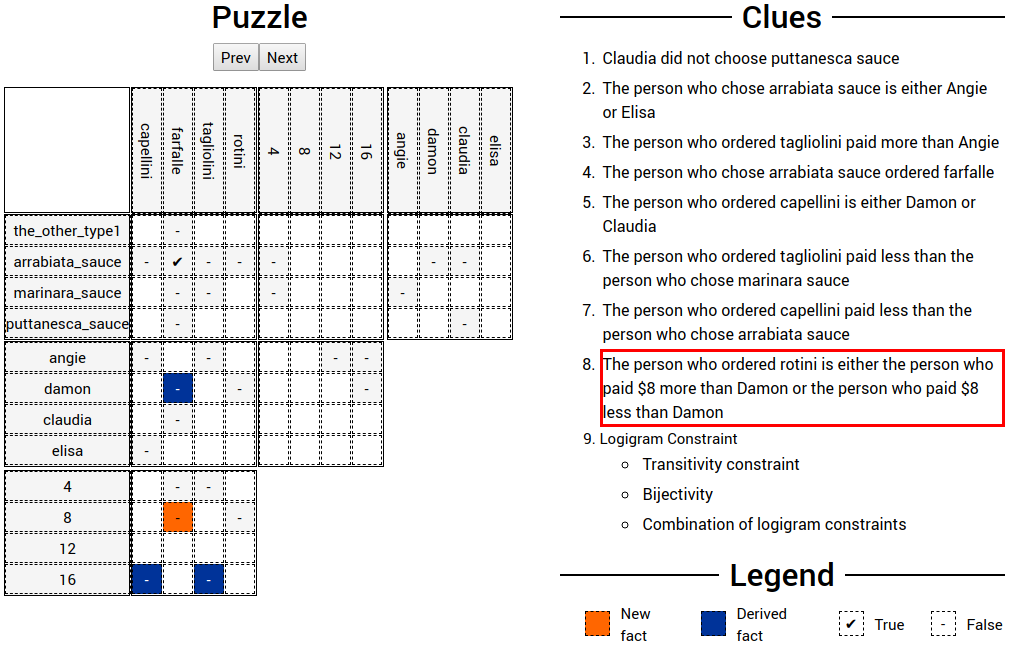
\includegraphics[width=\linewidth]{figures/zebra_screen_2}
\caption{Demonstration of hard explanation.}
\label{fig:screen2}
\end{figure}
\bart{Screenshot quality}


Intuitively, the reasoning happening here can be explained as follows: if \textit{farfalle} were to cost \$8, then due to the assumptions and bijectivity \textit{rotini} would cost 16. However, since Damon did not take \textit{farfelle} (which we assumed costs \$8), this is in contradiction with the highlighted clue. Hence \textit{farfalle} does not cost \$8. 
}

